\documentclass[a4paper, 11pt]{article}

% Nécessaire
\usepackage[french]{babel}
\usepackage[utf8]{inputenc}
\usepackage[T1]{fontenc}
\usepackage{lmodern}
\usepackage{amsmath, amsthm}
\usepackage{amsfonts,amssymb}

% Marge
\usepackage{geometry}
\geometry{margin={2.2cm ,2cm}}

% Figures, graphiques
\usepackage{graphicx}
\usepackage{epsfig}
\usepackage{caption}

% Surlignage
\usepackage{alltt}

\usepackage{xcolor}
\usepackage{soul}
\usepackage{color}
\usepackage{colortbl}

% Indicatrice
\usepackage{dsfont}

\usepackage{multirow}
\usepackage{eurosym}
\usepackage{extarrows}

% Graphique
\usepackage{tikz}


% Titre
\title{ACP sur les résultats donnés par NSGA-II}
\author{}
\date{}



\begin{document}
\maketitle   

L'algorithme NSGA-II a été repété 5 fois avec une taille de population égale à 100. Parmi les 500 jeux de paramètres obtenus, seuls 317 se trouvaient effectivement sur le front de Pareto.
Il faut donc sélectionner la solution qui nous convient le mieux --- aucune solution en domine une autre.

L'idée est alors de réaliser une ACP sur nos 317 résultats, avec comme variables principales nos trois critères et les valeurs des cinq paramètres en tant que variables supplémentaires.

\section{ACP}

Nous avons seulement trois composantes. On ne sélectionnera que les deux premières qui capturent à elles deux près de 91\% de l'inertie. Les représentations des individus et des variables sont visibles sur la figure~\ref{fig:pca}.

\begin{figure}[ht]
 \centering
 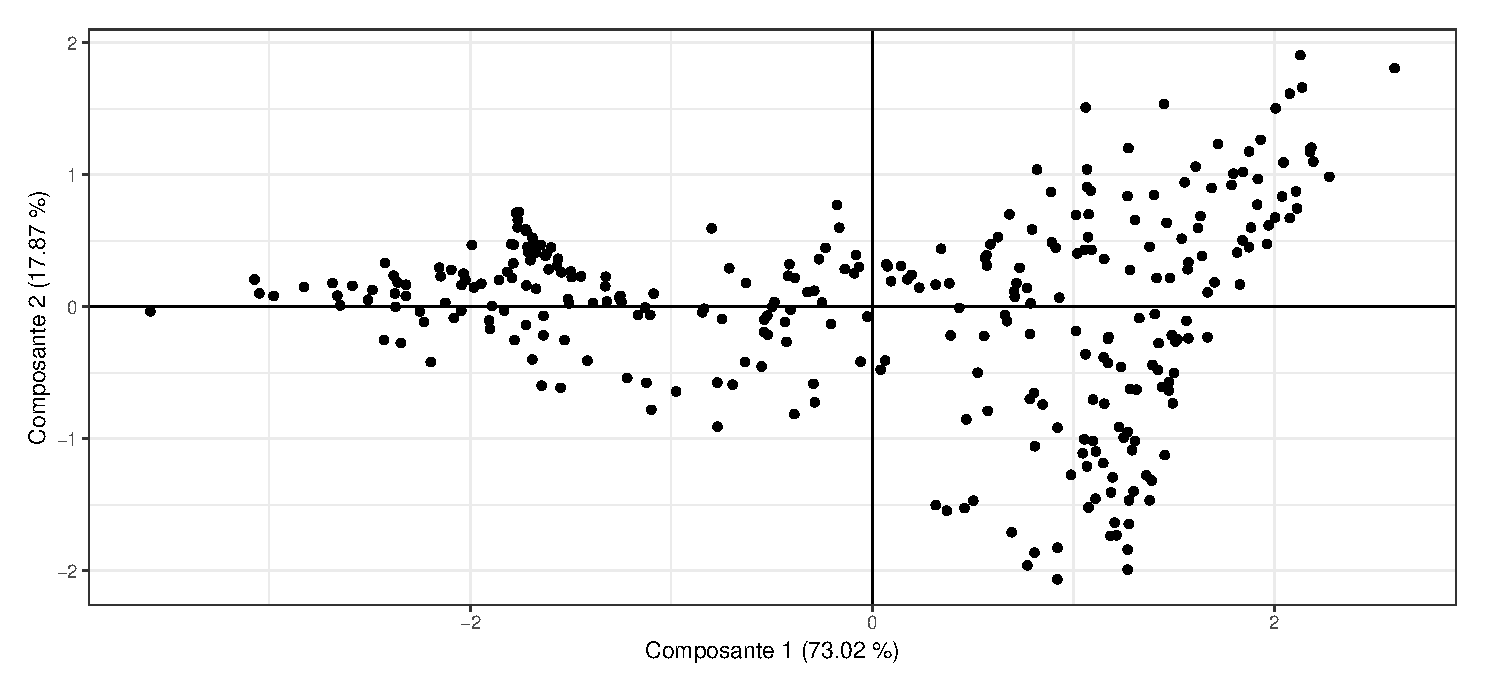
\epsfig{file = plots/pca_nsga_ind.eps, scale = 0.65}
 
 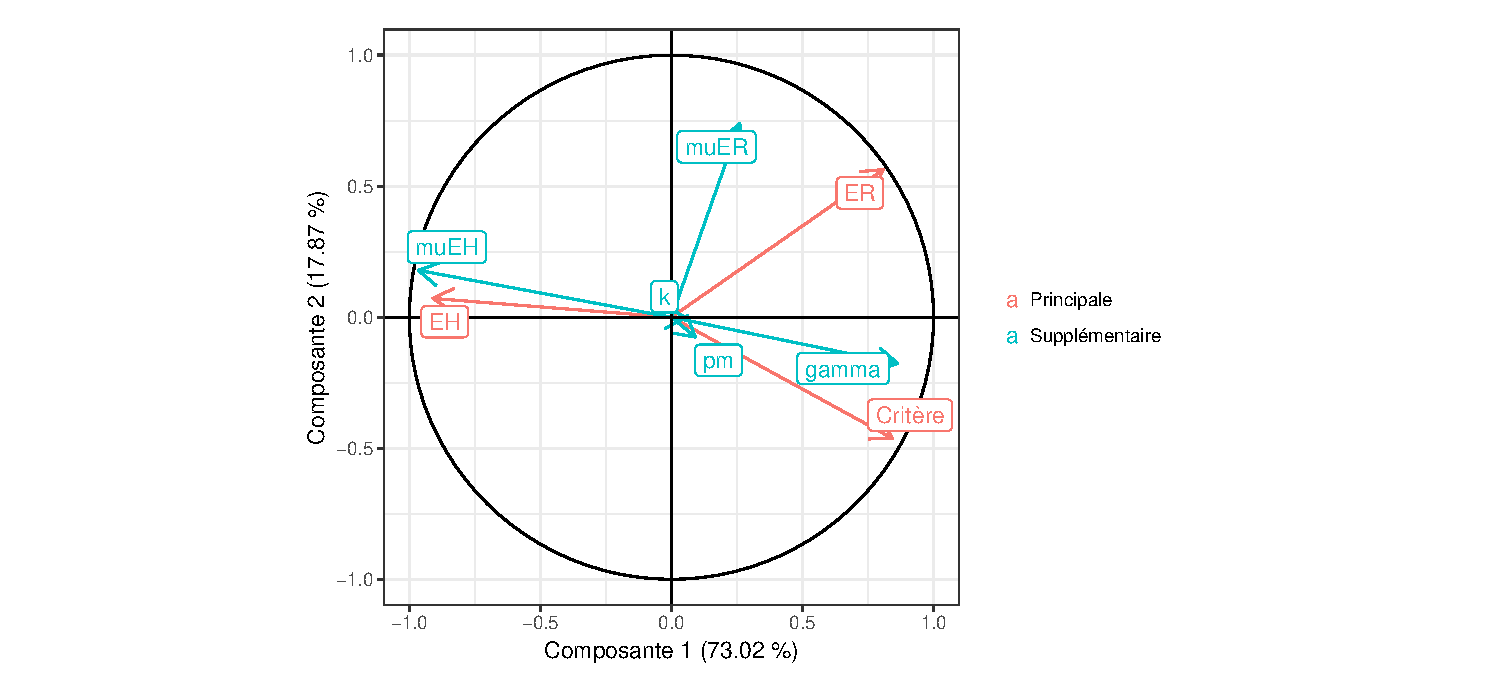
\epsfig{file = plots/pca_nsga_var.eps, scale = 0.65}
 
 \caption{Repésentation des individus (en haut) et des variables (en bas) sur le plan (1,2).}
 
 \label{fig:pca}
\end{figure}

On remarque d'emblée que certaines de nos solutions (les individus de l'ACP) privélgient un critère aux autres. \textit{A priori} ces solutions-là ne sont pas celles qui nous intéresse le plus, vu que l'on voudrait plutôt des paramètres qui ne négligent aucun des critères; nous sommes donc plus à la recherche d'un compromis. Certaines des paramètres sont corrélés à nos critères. Ainsi le paramètre $\mu_{EH}$ est corrélé au critère ER et le critère Critère est corrélé à $\gamma$. Le critère ER est quant à lui plus ou moins corrélé au paramètre $\mu_{ER}$.


Parmi les solutions, on s'intéresse au solutions qui :
\begin{itemize}
 \item un $\mu_{ER}$ supérieur à la médiane des $\mu_{ER}$ de toutes les solutions ;
 \item un $\mu_{ER}$ supérieur à la médiane des $\mu_{ER}$ de toutes les solutions ;
 \item un $\gamma$ inférieur à la médiane des $\gamma$ de toutes les solutions ;
 \item un $p_m$ supérieur à la médiane des $p_m$ de toutes les solutions.
\end{itemize}
Les solutions correspondant à ces critères sont visibles sur la figure~\ref{fig:sol}.


\begin{figure}[ht]
 \centering
 
 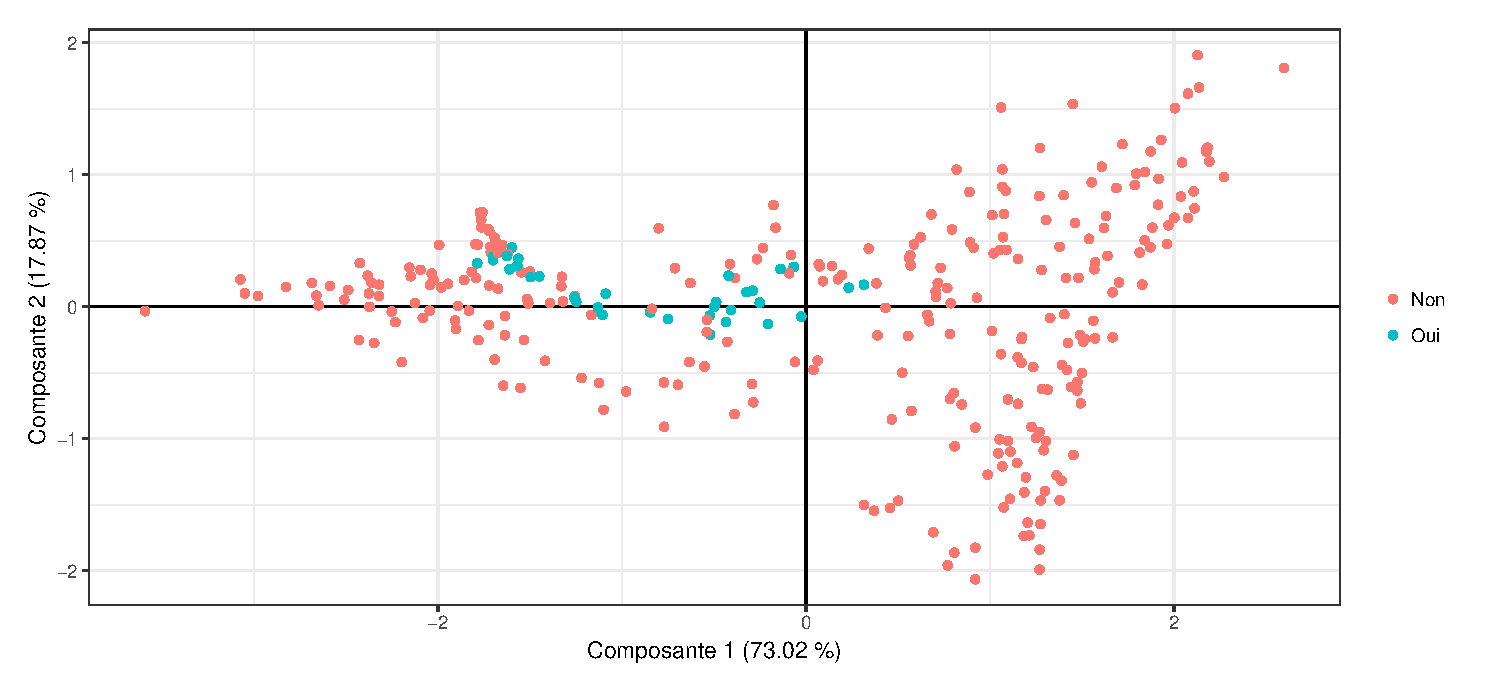
\epsfig{file = plots/ind_pca_ok.eps, scale = 0.65}
 
 \caption{Repésentation des individus sur le plan (1,2) correspondant aux solutions les plus intéressantes \textit{a priori}.}
 
 \label{fig:sol}
\end{figure}

Trente-cinq solutions sont ainsi retenues. On essaye deux jeux de paramètres : celui qui minimise la norme 1 et celui correspondant à la moyenne des 35 solutions. Les paramètres sont
{%
\newcommand{\mc}[3]{\multicolumn{#1}{#2}{#3}}
\begin{center}
\begin{tabular}{lllll}
\mc{5}{c}{Min $\|\cdot \|_1$}\\
$\gamma$ & $p_m$ & $\mu_{ER}$ & $\mu_{EH}$ & $k$\\
0.042 & 0.960 & 0.999 & 0.408 & 1.563\\
\mc{5}{c}{Moyenne}\\
$\gamma$ & $p_m$ & $\mu_{ER}$ & $\mu_{EH}$ & $k$\\
0.031 & 0.978 & 0.981 & 0.625 & 20.760
\end{tabular}
\end{center}
}%
Les dynamiques associées sont visibles sur la figure~\ref{fig:dyn}.
\begin{figure}[ht]
 \centering
 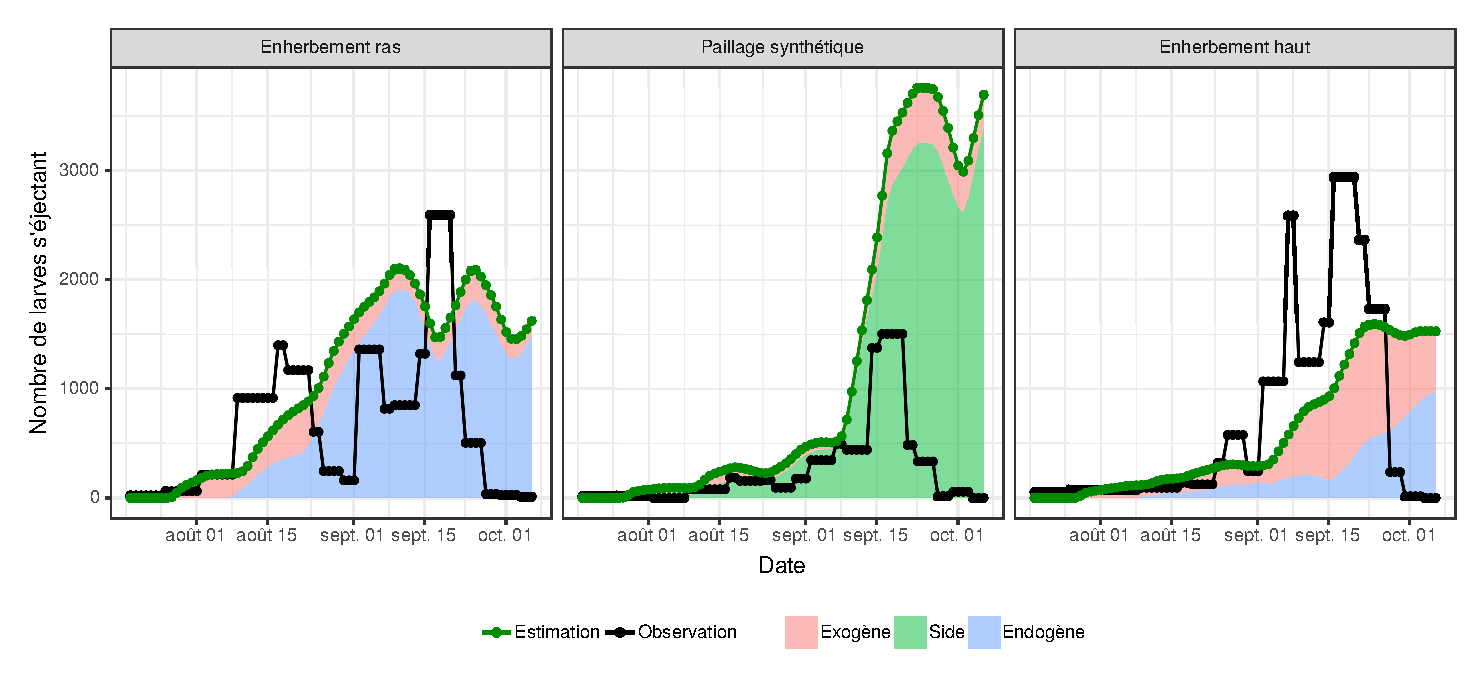
\epsfig{file = plots/arg1.eps, scale = 0.65}
 
 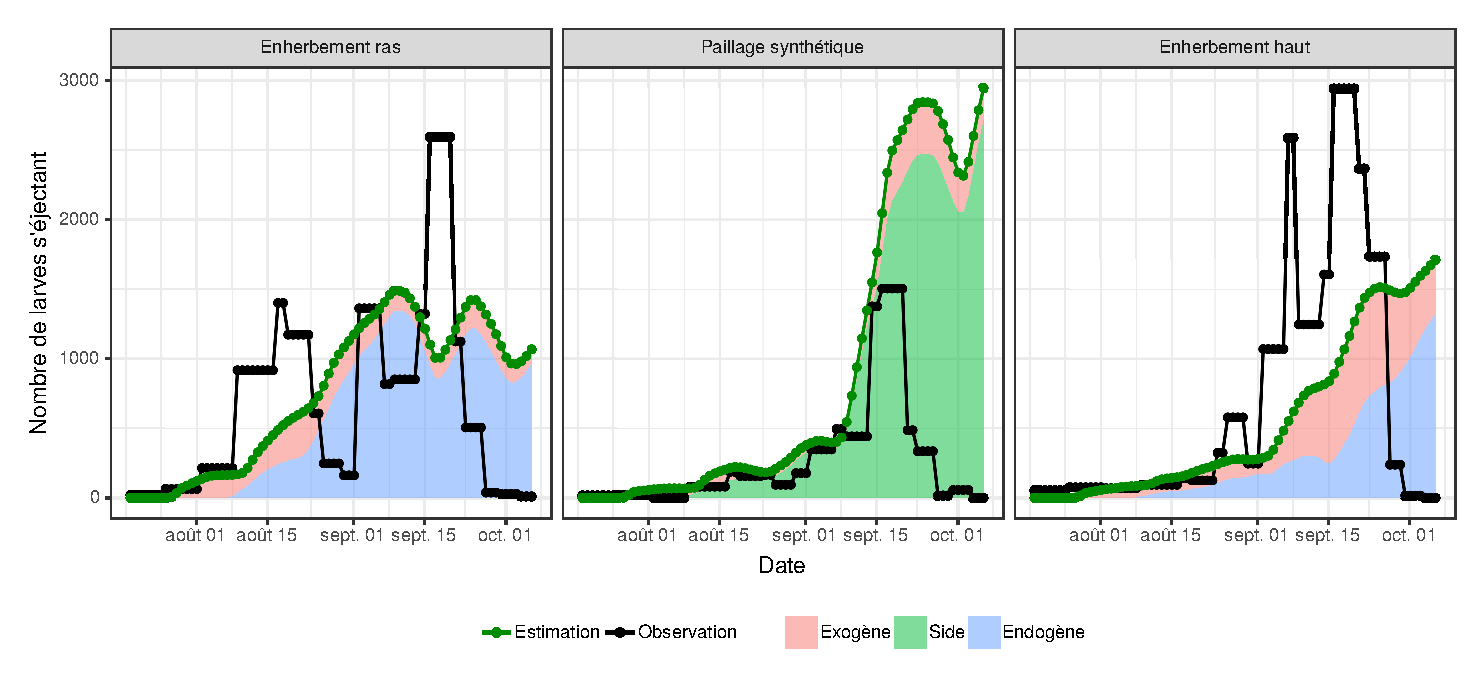
\epsfig{file = plots/arg2.eps, scale = 0.65}
 
 \caption{Dynamiques produites par la minimisation de la norme 1 (en haut) et par la moyenne des solutions retenues (en bas).}
 
 \label{fig:dyn}
\end{figure}



















\end{document}
